%!TeX program = xelatex
\documentclass[12pt,hyperref,a4paper,UTF8]{ctexart}
\usepackage{RUCReport}
\usepackage{listings}
\usepackage{xcolor}
%\usepackage{subfigure}
%\usepackage{subcaption,caption}
\usepackage{graphicx}
% 定义可能使用到的颜色
\definecolor{CPPLight}  {HTML} {686868}
\definecolor{CPPSteel}  {HTML} {888888}
\definecolor{CPPDark}   {HTML} {262626}
\definecolor{CPPBlue}   {HTML} {4172A3}
\definecolor{CPPGreen}  {HTML} {487818}
\definecolor{CPPBrown}  {HTML} {A07040}
\definecolor{CPPRed}    {HTML} {AD4D3A}
\definecolor{CPPViolet} {HTML} {7040A0}
\definecolor{CPPGray}  {HTML} {B8B8B8}
\definecolor{keywordcolor}{rgb}{0.8,0.1,0.5}
\definecolor{webgreen}{rgb}{0,.5,0}
\definecolor{bgcolor}{rgb}{0.92,0.92,0.92}

\lstset{
    breaklines = true,                                   % 自动将长的代码行换行排版
    extendedchars=false,                                 % 解决代码跨页时,章节标题,页眉等汉字不显示的问题
    columns=fixed,       
    numbers=left,                                        % 在左侧显示行号
    basicstyle=\zihao{-5}\ttfamily,
    numberstyle=\small,
    frame=none,                                          % 不显示背景边框
    % backgroundcolor=\color[RGB]{245,245,244},            % 设定背景颜色
    keywordstyle=\color[RGB]{40,40,255},                 % 设定关键字颜色
    numberstyle=\footnotesize\color{darkgray},           % 设定行号格式
    commentstyle=\it\color[RGB]{0,96,96},                % 设置代码注释的格式
    stringstyle=\rmfamily\slshape\color[RGB]{128,0,0},   % 设置字符串格式
    showstringspaces=false,                              % 不显示字符串中的空格
    % frame=leftline,topline,rightline, bottomline         %分别对应只在左侧,上方,右侧,下方有竖线
    frame=shadowbox,                                     % 设置阴影
    rulesepcolor=\color{red!20!green!20!blue!20},        % 阴影颜色
    basewidth=0.6em,
}

\lstdefinestyle{CPP}{
    language=c++,                                        % 设置语言
    morekeywords={alignas,continute,friend,register,true,alignof,decltype,goto,
    reinterpret_cast,try,asm,defult,if,return,typedef,auto,delete,inline,short,
    typeid,bool,do,int,signed,typename,break,double,long,sizeof,union,case,
    dynamic_cast,mutable,static,unsigned,catch,else,namespace,static_assert,using,
    char,enum,new,static_cast,virtual,char16_t,char32_t,explict,noexcept,struct,
    void,export,nullptr,switch,volatile,class,extern,operator,template,wchar_t,
    const,false,private,this,while,constexpr,float,protected,thread_local,
    const_cast,for,public,throw,std},
    emph={map,set,multimap,multiset,unordered_map,unordered_set,
    unordered_multiset,unordered_multimap,vector,string,list,deque,
    array,stack,forwared_list,iostream,memory,shared_ptr,unique_ptr,
    random,bitset,ostream,istream,cout,cin,endl,move,default_random_engine,
    uniform_int_distribution,iterator,algorithm,functional,bing,numeric,},
    emphstyle=\color{CPPViolet}, 
}

\lstdefinestyle{Java}{
    language=[AspectJ]Java,
    keywordstyle=\color{keywordcolor}\bfseries
}

\lstdefinestyle{Python}{
    language=Python,
}

%%-------------------------------正文开始---------------------------%%
\begin{document}

%%-----------------------封面--------------------%%
\cover

%%------------------摘要-------------%%
%\begin{abstract}
%
%在此填写摘要内容
%
%\end{abstract}

\thispagestyle{empty} % 首页不显示页码

%%--------------------------目录页------------------------%%
\newpage
\tableofcontents
\thispagestyle{empty} % 目录不显示页码

%%------------------------正文页从这里开始-------------------%
\newpage
\setcounter{page}{1} % 让页码从正文开始编号
%%可选择这里也放一个标题
\begin{center}
   \title{ \Huge \textbf{{早期轴承微小故障失效分析与诊断}}}
\end{center}

\section{背景介绍}

\subsection{项目背景及意义} 
随着社会不断地的向前发展,现代工业的生产力急剧上升,工业4.0与智能制造的概念正逐步落地。与此同时,机械设备正朝着高速、精密、大型及智能方向快速发展,机械设备呈现出规模大、结构复杂的形态,其内部各部件之间的动力学耦合效应日益显著。自然地,此种形态导致与机械设备工作状态相关的内、外因素数量增加,映射关系更加复杂多样,给系统的稳定性带来了严峻挑战。若实际工况中,机械设备由于关键元件故障而产生级联效应,极易导致生产秩序紊乱,继而造成巨大的经济损失和重大事故发生,甚至人员死伤[1]。旋转机械作为机械设备中举足轻重的构成部件,是动力传输与执行的核心,被广泛应用于制造、医疗及能源等各个行业,故其状态监测与故障诊断是机械领域的重点。在诸多旋转机械中,滚动轴承作为不可或缺的构件,被视为用于动态元件和固定元件连接的“关节”,承载着降低摩擦系数与保证回转精度的重任。此外,因其装配方便、效率高、摩擦阻力小、润滑容易实现等优点,在旋转机械中广泛应用[2-3]。

作为实际工况中使用频率最高的必不可少的设备,滚动轴承也因其承载环境复杂而成为发生故障最频繁的元件之一。因此,其运转状态通常直接关系到整个设备的精度、可靠性及寿命[4-5]。但在实际工程中,滚动轴承在机械设备中起承受载荷和传递载荷作用,工作条件最为恶劣,常处于高速、重载、高温及强冲击的复杂环境下。由于其工作面长期受到赫兹接触应力(Hertzian Contact Stress)的反复作用,材料内部极易产生疲劳积累,进而极大概率会诱发磨损、浸蚀及裂纹等失效形式[6]。若已诱发的失效未能及时得到维修,随着运转时间的推移,微小损伤会迅速扩展,进一步发展导致轴承断裂、抱死甚至彻底丧失功能,从而引发灾难性事件。据有关资料统计,由滚动轴承失效导致的电机故障率约为44\%,约有20\%齿轮箱故障是轴承故障诱发。此外,机械故障中,70%左右源于振动故障。在振动故障中,约30%故障的诱因是轴承失效[7]。这些数据充分表明,滚动轴承是旋转机械系统中最为薄弱且关键的环节。

以此可推断,滚动轴承安全平稳运转是保证机械设备乃至整个生产工况有条不紊运行的必要前提和关键因素。为此,针对滚动轴承工作状态的有效监测和诊断手段需不断探索,从传统的“事后维修”向“预测性维护”(Predictive Maintenance)转变,以便更准确把握其故障产生和演变机理,旨在及时挖掘潜藏故障,规避机械设备重大故障的发生,进而避免人力和物力的巨大损失,具有显著的经济效益和安全效益。此外,滚动轴承由于其工作条件恶劣不但是易损零件,而且寿命具有很大的离散性,即便是同一批次的产品在相同工况下,其剩余使用寿命(RUL)也可能存在巨大差异,故滚动轴承与许多旋转机械中的故障相关联。总结来说,探索和研究滚动轴承的状态监测与诊断方法,对于保障大国重器的安全运行,在理论研究和实际运用层面都极具意义。

虽然轴承故障诊断技术日趋成熟,基于振动分析、声发射及电流信号的诊断手段层出不穷,但绝大多数方法只能诊断出特征明显的重大故障或晚期故障。遗憾的是,在实际过程中,当轴承的运行状态发生异常时,如存在微点蚀、微裂纹等微小故障(Incipient Faults)时,故障激发的冲击响应极其微弱。此时,轴承振动加速度信号时常存在幅值低、信噪比极低、且易被齿轮啮合频率、环境噪声等未知扰动掩盖而导致故障特征信号不明显的特点,给轴承运行状态的安全监控造成了极大困难。然而,轴承显著性故障都起源于微小故障,故障的演化往往经历一个非线性累积的过程,若可及时诊断轴承微小故障,可有效预防重大事故发生,减少巨大的轴承损坏造成的损失,实现全寿命周期的健康管理。因此,针对轴承故障特征不明显的微小故障采取相应方法进行故障特征提取及诊断,通过先进的信号处理算法剥离强噪声背景,以保证轴承故障诊断及安全监控的精确性,受到国内外学者的极大重视[8-9]。 \par

\par
探究轴承故障可能原因并进行轴承失效分析,不仅可以积累发现和诊断轴承故障的经验,以保证机械系统的稳定性、可靠性和寿命,同时也可以降低维护成本,提高工作效率。
因此本报告将以滚动轴承为研究对象,将从宏观及微观角度进行失效分析。

\begin{figure}[htbp]
	\centering
	% 修复:使用 subcaptionbox 替代 subfigure
	\subcaptionbox{滑动轴承}{
		\includegraphics[width=0.3\linewidth]{figures/C1/plain_bearing.jpg}
	}
	\quad % 空格
	\subcaptionbox{滚动轴承}{
		\includegraphics[width=0.3\linewidth]{figures/C1/bearing1.jpg}
	}
	\caption{不同类型的轴承}
	\label{p1}
\end{figure}

\subsection{轴承分类及工作原理} 
滚动轴承微小故障诊断仍旧面临诸多的困难和阻碍,信号特征微弱且非平稳特性显著,单纯依赖信号处理算法往往难以触及本质。因此,需在已有框架基础上进一步构建更精确的诊断模型,而对滚动轴承的动力学行为及故障演变机理展开深入研究,是实现微小故障精细化诊断的必要前提。物理结构的理解是建立故障模型的基础,因此,本报告首先就滚动轴承的基本分类、结构组成以及运动学机理展开讨论。

从摩擦性质的维度来看,轴承主要分为滑动轴承(Sliding Bearing)和滚动轴承(Rolling Element Bearing)两大类,如图~\ref{p1}所示。滑动轴承依靠轴颈与轴瓦之间的滑动摩擦工作,通常在工作面间形成流体动压或静压油膜以承载负荷,广泛应用于重载、高精度的场景。而滚珠轴承和滚柱轴承统称为滚动轴承,是工业现场最为标准化的精密机械元件。滚动轴承通过引入滚动体,将轴与轴座之间的滑动摩擦转化为滚动摩擦,从而显著降低了摩擦系数。这种机制使得滚动轴承能够在极低的启动力矩下运行,并适用于从低速重载到高速轻载的广泛工况,展现出卓越的耐久性和互换性。滚动轴承通常由四个核心部分组成:一个外圈、一个内圈、在重动载荷和相对高速下接触的滚动元件,以及用于隔离并引导这些滚动元件的保持架。

滚动轴承在实际工况中起到“关节”的重要作用,限制了转子的径向和轴向自由度,是现代生产设备必不可少的部件之一。滚动轴承的基本架构主要包括内圈(Inner Ring)、外圈(Outer Ring)、滚动体(Rolling Elements)和保持架(Cage)四个部件,其整体拓扑结构和详细剖面见图~\ref{p3}。

在具体的机械系统装配中,各部件承担着特定的运动学与动力学功能: \begin{enumerate} \item \textbf{内圈与外圈}:通常情况下,外圈与轴承座或箱体孔配合,在运行时处于静态或相对静态,起支撑作用;内圈则通过过盈配合固定在旋转轴的轴颈上,随轴一同高速旋转。为优化接触应力分布并限制轴向位移,内、外圈表面均加工有高精度的凹槽滚道(Raceway)。滚道是滚动体运行的轨迹,其曲率半径的设计直接影响接触面积与承载能力。 \item \textbf{滚动体}:作为衔接动态部件(内圈)和静态部件(外圈)的核心介质,滚动体是承受并传递载荷的关键。根据承载需求的不同,滚动体被设计为球形(点接触)或圆柱形、圆锥形(线接触)。其几何尺寸、数量及形状精度直接决定了轴承的额定动载荷、刚度及极限转速。 \item \textbf{保持架}:又称保持器,其主要作用是将滚动体均匀地分隔在滚道周围,防止滚动体之间发生直接接触、碰撞或集聚,从而避免摩擦力矩的剧烈波动。同时,保持架还起到引导滚动体运动、改善内部润滑条件的作用,对于高速旋转下的稳定性至关重要。 \end{enumerate} 正是这种精密的配合结构,使得滚动轴承在极小的摩擦损耗下实现了运动传递。然而,这也意味着一旦任一部件表面出现微小损伤,都会破坏原有的弹性流体动力润滑(EHL)状态,进而激发周期性的冲击振动。

\begin{figure}[htbp]
	\centering
	\includegraphics[width=0.6\linewidth]{figures/C1/bearing3.jpeg}
	\caption{滚动轴承结构示意图}
	\label{p3}
\end{figure}


\subsection{轴承的主要失效形式}
滚动轴承是生产过程中最常使用的部件之一,但在实际长期运行过程中,由
于载荷下各部件的相互摩擦、恶劣的工况环境及安装工艺欠佳等缺陷,不可避免
地出现故障。随着其不断运行,故障程度不断的积累,最终将会发生重大故障,
直接影响轴承运行状态,继而令轴承完全失效,造成设备严重损坏。如图~\ref{p5}所示,滚动轴承的
故障主要包括以下几种形式。

(1)磨损失效

磨损失效是滚动轴承故障形式中出现频率最高的一种故障形态。在滚动轴承
的工作过程中,滚动体随着其运转不断地在内、外圈间的滑槽滑动,长期的滑动
导致部件表面出现磨损。此外,在滚动轴承负荷运行时,若金属粉末或者其它坚
硬杂物误入轴承内部,将会对轴承工作表面造成一定程度的磨损。

(2)疲劳失效

疲劳失效时常发生于轴承的表面。由于滚动体表面和滚道长期承受着重物和
相互挤压的压力,导致在最大剪应力处形成裂纹。裂纹是疲劳失效最初期的故障
体现,裂纹进一步发展则成为剥落坑,最终导致剥落从而引起轴承失效,这种失
效即疲劳失效。

(3)腐蚀失效

腐蚀失效是由金属部件松动、缝隙夹渣和表面缺陷等诱发的微电池作用而触
发。点腐蚀是腐蚀的初期症状,随着腐蚀面的不断扩大,最终造成表面剥落使轴
承失效,即腐蚀失效。

(4)塑性变形失效

轴承在运行中,若遭受较大的冲击负荷或者坚硬颗粒杂物的侵入,将会导致
轴承部件表面的凹痕、划痕或压痕的产生,称之为塑性变形。随着这种变形的不
断增大,最终将引起剥落导致轴承失效,即塑性变形失效。

(5)胶合失效

由于高转速、重负荷、润滑程度不足,轴承会因为摩擦产生巨大而短暂的温
度,导致部件表面烧损。在这种巨大的温度下,滚动体和滚道的局部表面粘连到
一起导致轴承失效,即胶合失效。

(6)断裂失效

在长时间运转过程中,滚动轴承会因为承力过大、转速太大、润滑程度不够、
加工误差或者安装不当产生超过其承受上限的热应力。正是因为这种过大的热应
力造成了轴承元件的断裂。

%%%%%%%
\begin{figure}[htbp]
	\centering
	% 修复:使用 subcaptionbox 替代 subfigure
	\subcaptionbox{轴承磨损}{
		\includegraphics[width=0.45\linewidth]{figures/C1/mo_sun.jpeg}
	}
	\quad
	\subcaptionbox{轴承裂纹}{
		\includegraphics[width=0.45\linewidth]{figures/C1/lie_wen.png}
	}
	\quad
	\subcaptionbox{轴承腐蚀}{
		\includegraphics[width=0.45\linewidth]{figures/C1/fu_shi.png}
	}
	\quad
	\subcaptionbox{轴承碎裂}{
		\includegraphics[width=0.45\linewidth]{figures/C1/sui_lie.jpeg}
	}
	\caption{轴承的主要失效形式}
	\label{p5}
\end{figure}

%%------------------------第二章从这里开始-------------------%
%% Part1:宏观断口分析(变形),微观断口分析(裂纹)
%% Part2:元素分析  
\section{项目介绍}
\subsection{现有资料分析}
轴承动力学模型是研究轴承运动和力学特性的重要工具,通过建立轴承的数
学模型来描述其运动和受力情况,可以实现对轴承性能的分析和优化。滚动轴承
仅由四个部件(即内圈、外圈、保持架和滚珠)组成,但在现实中,滚动轴承的
静态和动态行为非常复杂。原因在于不同轴承部件之间的非线性接触以及轴承运
行过程中出现的复杂摩擦机械现象。因此,滚动轴承建模对于获得基本原理的知
识至关重要。在过去的几十年里,许多模型已经可以用于滚动轴承的设计和仿真。
目前,轴承动力学模型的研究已经在国内外取得了非常多的研究成果。下面将从
正常轴承的建模、局部缺陷建模和打滑轴承的建模三个方面进行综述。

首先,就滚动轴承的正常模型而言,国内外研究者已经有大量成熟的研究成
果了。归纳总结,可以将滚动轴承模型分为集总参数模型、准静态模型、准动态模
型、动力学模型和有限元模型[10]。动力学模型会更加接近轴承的运动状况。在动态
模型中,不使用静态约束。所有的过渡和旋转运动用微分方程描述。对于这方面的
研究很早就开始了,瑞典的SKF 公司和美国Franklin 研究所合作拉开了对轴承动
力学的研究,提出了基于套圈控制理论的自由圆环弯曲振动模型[11]。文献[12]提出了滚珠轴承和滚柱轴承最具代表性的动力学模型之一。滚珠轴承中的三种主要
相互作用以及滚柱轴承中的四种主要相互作用。

其次,在正常的轴承研究之上,有学者对滚动轴承局部缺陷特征的动力学模
型进行了大量的研究。文献[8]提出了用半正弦函数和三角函数描述缺陷区
滚动元件运动状态的数学建模方法。文献[9]提出了一种基于矩形脉冲函数表
征轴承缺陷冲击特性的方法。他们在模型中考虑了缺陷位置的影响。文献[10]使用切线和矩形函数来描述缺陷轴承的偏转激励。文献[11]提出了一
种计算带有矩形缺陷的双列轴承准静态载荷分布和变刚度的方法。文献[12]建
立了一种通过计算滚动元件通过矩形缺陷的位移来估计滚动轴承缺陷大小的方法。
文献[13]与[14]将缺陷特征描述为一个锋利的矩形。

最后,还有学者关注轴承动力学分析的分支打滑现象。该部分研究者考虑了
实际情况下的轴承打滑现象,对轴承的打滑行为做了研究分析。轴承打滑是代表轴承动态性能的另一个重要指标,在轴承运行中经常观察到。它很可能对滚动元件和滚道造成划痕和磨损,并严重影响轴承的工作性能和使用寿命,
特别是在剧烈的载荷振荡和快速的速度变化下。因此,随着研究工作的深入和深入,轴承
打滑现象越来越受到人们的重视。
\subsection{失效初步原因诊断}
如图\ref{f1} 所示, 轴承在正常使用一段时间后突然发生失效
断裂,我们项目组对本次失效提出了我们的问题,本次失效是由于疲劳断裂、过载断裂、腐蚀断裂还是材料工艺原因导致的断裂?

\begin{figure}
	\centering
	\includegraphics[width=0.6\linewidth]{figures/C2/1.jpg}
	\caption{轴承失效断裂}
	\label{f1}
\end{figure}
轴承零件中的任何一个都可能出现故障,这些故障通常是单点缺陷,如切屑
或凹痕。当这些元件相互移动时,这些缺陷与轴承中的其他元件周期性接触,并且
在每个接触处,它们可以在整个结构中激发高频共振。滚动轴承损坏可能导致滚
动轴承降低工作效率甚至完全失效。只有当运行和环境条件以及轴承布置的细节
完全一致时,轴承布置才能有效运行。轴承损坏并不总是由轴承本身造成的。由
于轴承材料或工艺缺陷造成的损坏属于例外。

初步讨论,我们组认为本次轴承失效的原因大概由以下几点:

(1) 润滑不足或污染:润滑不足或使用了不合适的润滑剂可能导致滚动轴承的过早失效。此外,当润滑油或脂中含有污染物时,也可能损伤轴承。

(2) 超载:超过轴承设计的额定负载或短时间内的大负荷可能导致轴承的损坏或过早的疲劳失效。

(3) 安装不当:如果轴承在安装时受到损伤、施加不均匀的载荷或存在对齐问题,可能会导致轴承的早期失效。

(4) 环境因素:如高温、湿度、化学物质(如酸、碱)等,可能会对轴承材料产生腐蚀或其他形式的损害。

(5) 外部污染:外部尘埃、金属屑或其他颗粒物可能进入轴承内部,导致轴承的磨损和损坏。

总之,我们初步得出结论,判定本次失效的主要为安装不当导致在安装时轴承受到损伤同时也受到了外部污染等化学因素的影响造成。
\subsection{本项目的短期解决方法}
在我们小组进行初步原因诊断后,我们立刻制定了短期解决措施,将本次失效损失降到最低。我们将从以下方面进行初步解决

(1) 更换轴承: 最直接的方法是更换失效的轴承。确保使用正确规格和品质的轴承来替换。

(2) 润滑处理: 如果发现轴承润滑不足或质量有问题,我们可以及时添加适当的润滑油或脂。确保润滑油或脂的品质和量都符合规定。

(3) 调整安装: 检查轴承的安装状态,确保其正确对中并且预紧力适当。如果需要,进行适当的调整或校正。

(4) 临时支撑: 在更换轴承之前,如果可能的话,可以考虑添加临时支撑或支撑结构,以减少负载并延长设备的使用寿命。

(5) 降低工作条件: 在进行修复之前,可以考虑降低负载、转速或其他工作条件,以减少对轴承的进一步损伤。

需要注意的是,虽然本报告通过采用以上的方法帮助暂时解决轴承断裂的问题并确保设备的正常运行,但本报告将会进一步对轴承的数学模型以及元素进行相应的分析,以避免未来的失效和损坏。
\subsection{本项目的长期解决方法}
本报告旨在利用数据分析和电镜检测相结合的方式,对滚动轴承的问题进行全面分析。近些年,制造行业一直在研究如何利用数学模型、计算机模拟和实验方法来优化轴承的设计。经过深入研究,总结出四种主要的轴承故障检测手段:振动监测、声学监测、温度监控以及磨损颗粒检查。特别是振动监测,其应用范围非常广泛。

在各种监测方法中,振动分析成为了最受欢迎的技术,因为每个轴承缺陷都会导致滚动部件的特定振动,从而产生连续的振动脉冲。这种振动不仅有低频部分,还有与冲击有关的高频组成。除了使用振动数据,许多研究者还研究了决定轴承行为的物理定律,并尝试用数学方程式来描述这些系统。此外,通过电镜技术,可以对轴承的结构、组件和细节进行详细观察和分析,从而更有效地预防轴承未来可能出现的故障和损伤。下面将对基于数据的故障诊断分析方法分类进行着重说明。

\subsubsection{轴承动力学建模}
本报告将首先对多自由度轴承动力学模型进行了详细介绍。随后,通过研究轴承波纹度、接触刚度以及赫兹接触力理论,建立具有两个自由度的轴承的正常动力学方程。此外,对局部故障下的轴承动力学模型进行了深入研究,运用分段函数揭示了球在经过故障部分时的激励过程,由此推导出了缺陷故障轴承的动力学方程。最终,采用四阶龙格库塔数值解法求解这一二阶方程。
\subsubsection{轴承的早期微小故障检测}
目前的文献研究表明,轴承的动力学模型展现出多输入频率和非线性的特性。基于这种非线性特性,我们可以对轴承的运动行为进行深入探究。在这种非线性体系中,确定了确切的输入频率及其数量后,可以进一步确定主要的输出频率。尽管存在众多输出频率,但与输入频率密切相关的输出频率往往携带了大部分的能量信息,这些输出频率的特征值相对较高。因此,这些核心输出频率可以代表整体的输出特性。
\subsubsection{输入频率未知的轴承故障检测}
当滚动体存在滑动摩擦时,滚动体的自旋速度无法简单地通过线性关系来确定。因此,本部分主要探讨的是在输入频率不确定的情况下的轴承故障检测。通过信号的采集,我们可以推断输出频率,尽管在已知非线性阶数的前提下,我们可能对基频一无所知,或者在非线性系统结构上并不清楚的情境下进行输入频率的估算和故障检测。该部分的核心挑战在于如何有效地利用互调结构来增强信号的估计能力。

\subsection{小结}
报告的第二部分对轴承现有分析方法、失效的初步原因诊断、本项目的短期解决方法以及本项目的长期解决方法进行了综述,同时针对目前研究内容的不足之处,本部分提出利用基于轴承动力学建模、早期微小故障诊断和频率未知下的轴承故障检测器的数据故障诊断方法和电镜观测的元素与端口分析方法结合的断裂分析方法,以避免轴承未来的失效和损坏。


%%------------------------第三章从这里开始-------------------%
\section{失效分析}

\subsection{轴承结构建模分析}
轴承结构建模是一个系统性的过程,用于描述和分析轴承的工作原理、性能和可能的问题。其包括:
(1) 基本几何建模:
基本几何建模包括考虑包括内圈、外圈、滚动体(如球或滚柱)、保持架和密封件的几何尺寸、形状和布局。
(2) 材料与物性分析:
该部分考虑轴承材料,如轴承钢、陶瓷等,以及它们的机械和热学性质(如硬度、弹性模量、热膨胀系数等)。
(3) 动力学建模:
该部分考虑轴承在运行时的动态行为,如旋转、振动和受力情况。使用多自由度系统动力学方程来描述轴承的动态行为。
(4) 摩擦和磨损分析:
该部分需要分析轴承中的摩擦现象,考虑摩擦力、热产生和可能的磨损模式。了解摩擦和磨损对轴承性能和寿命的影响。

在轴承研究的解析模型部分,动力学模型的构建是一个核心焦点。目前,轴承动力学模型涵盖了多种类型,如静力学模型、动力学模型、非线性模型以及有限元模型。具体来说,静力学模型主要关注轴承的受力分析,而不涉及其运动状态;有限元模型则针对轴承结构进行深入分析和设计;动力学模型考虑到轴承的实际运动,帮助研究其在不同操作条件下的振动行为和动态反应;而非线性模型则更适用于在高速和大负荷等特殊条件下探究轴承的非线性属性。

在本报告中,我们专注于对轴承的动态特性进行建模。初步阐述了轴承的内部工作机制,并基于轴承的运动状态、表面波纹度、接触刚度和Hertz接触力等要素,制定了二阶动力学方程。进一步地,我们深入研究了在故障情境下的动态方程。特别关注了由于局部缺陷导致的球与内外滚道之间的位移变动,揭示了这种位移如何引发振动响应的过程。这些分析为轴承故障检测提供了坚实的理论基础和数据支撑。

\subsubsection{正常模型的分析}
尽管滚动轴承的几何设计非常精确,但在运行时仍然会出现振动现象。这主要归因于滚动体与内、外圈之间的有限滚动接触,这些接触点具有其固有的弹性特性。为了深入理解轴承的动态行为,我们可以建立一个专注于其正常运行时的动力学模型。这种动力学模型在考虑到一些假设和简化前提后,通常分为单自由度和多自由度的系统模型。

1、单自由度系统模型

在单自由度系统模型中,我们将轴承系统简化为一个独立的质点的动态模型。这种简化模型假设在水平方向上,轴承系统可以被视为一个单一质点的运动,并且这个质点会受到外部载荷的影响。其具体的运动模式如下:
\begin{equation}
	m\ddot{x}+c\dot{x}+kx=F(t)
\end{equation}
其中,$m$是质点的质量;$x$是质点的位移;$\dot{x}$和$\ddot{x}$分别是质点的速度和加速度;$c$是阻尼系数;$k$是刚度系数;$F(t)$是外部载荷。


这种模型常被称为“二阶动力学模型”,因其基于二阶微分方程描述。为了确定这个模型的参数,我们可以利用实验技术和数学分析工具进行识别。

2、多自由度系统模型

多自由度系统模型描述了轴承系统不能被简化为单一质点运动的情况。相反,它包含多个相互作用的组件和多个质点。相对于单自由度系统模型而言,多自由度系统模型更为复杂。

通过使用拉格朗日方程,我们可以建立多自由度系统模型,并通过求解该模型得到系统的自然频率、阻尼和刚度等参数。多自由度系统模型的主要优势在于它能够考虑轴承系统中多个部件之间的相互作用,从而更准确地描述轴承的动力学行为。
\begin{figure}[!ht]
	\centering
	\includegraphics[width=0.6\linewidth]{figures/C3/fig3 modelZN.eps}
	\caption{轴承简化结构模型}
	\label{fig:轴承简化结构模型}
\end{figure}



轴承正常动力学模型的构建可以采用单自由度系统模型或多自由度系统模型。这些模型能够更全面地反映轴承系统的动力学特性。

滚动轴承的动力学模型直接由滚动体与滑道之间的接触特性决定。尽管滚动轴承的组件相对简单,但其内部运动和变形接触却十分复杂,尤其在制造工艺误差的影响下,波纹度会影响各组件之间的相对运动。当轴承发生故障时,其运动模型也将相应改变。因此,本部分研究了由加工误差引起的波纹度和缺陷对球和滚道之间接触特性的影响,以推导轴承的动力学方程。轴承的主要构件包括外圈、内圈、球和保持架,它们的简化结构模型可以分别描述其功能和相互作用。


\subsubsection{波纹度影响}

滚动轴承的振动主要与其波纹度有关。在轴承工作时,位于内外圈之间的滚动体(在此指为球体)会产生圆周式的移动。然而,由于制造过程的限制,内外圈和滚动体的表面并不是完全平滑的。因此,真正的圆周移动只会在完全光滑的轨道上实现,而在现实中考虑到波纹度时,球与轨道的接触会导致接触角的变化以及接触面曲率半径的变更,从而影响接触应力的分布。图~\ref{fig:波纹度模型}展示了轴承部件外表面的整体正弦形状的波纹度模型,其中波纹度的特征波长远远大于球与导向环之间赫兹接触面积的尺寸。我们用波数表示每周长波的数量。波纹度缺陷的存在揭示了球在轨道上运动的实际轨迹,明显表明其不是严格意义上的圆周运动,而是伴随着曲率变化的运动。



波纹度会使轴承在运行时的接触载荷发生变化。这种变化的程度与波纹度的深度和接触点的刚度密切相关。由于这种接触载荷的波动,轴承会出现振动。以下是外圈与第$j$个球接触点的波纹度数值:
\begin{equation}
	\label{eq2:波纹度1}
	P_{oj} = p_{m}\sin{[N_{o}(\omega_{c}t+\frac{2\pi(j-1)}{Z})+\eta_{o}]}
\end{equation}
式中$\omega_{c}$为保持架(Cage)的旋转角速度,$p_m$为外圈波纹度最大幅值,$N_o$是外圈的$N$个波纹,$Z$表示球的个数,$\eta_{o}$则是外圈波纹度的初始相位角。
同理内圈与第$j$个球接触处的波纹度值是:
\begin{equation}
	\label{eq2:波纹度2}
	P_{i j}=A_i \sin \left[N_i\left(\left(\omega_c-\omega t\right) t+\frac{2 \pi(j-1)}{Z}\right)+\beta_0\right]
\end{equation}
式中$A_i$表示内圈波纹度的最大幅值,$\omega_c$ 是保持架旋转速度,$\omega$ 是主轴旋转速度,$\beta_0$是内圈波纹度的初始相位角,$q_m$是内圈波纹度最大幅值。那么对于球而言,它同时和内圈和外圈接触,并且两者在相位上相差$\pi$,因此球在接触点处的波纹度值为:
\begin{equation}
	\label{eq2:波纹度3}
	u_{b j}=A_{m}\left[\sin \left(N_{b} \omega_{b}+\gamma_{0}\right)+\sin \left(N_{b}\left(\omega_{b}+\pi\right)+\gamma_{0}\right)\right]
\end{equation}
其中 $\omega_b$是球自转速度, $\gamma_0$为球波纹度值得初始相位角, $A_m$是球波纹度最大值。
\begin{figure}
	\centering
	\includegraphics[width=0.55\linewidth]{figures/C3/fig2.jpg}
	\caption{波纹度模型}
	\label{fig:波纹度模型}
\end{figure}

\subsubsection{接触刚度}
接触刚度受接触面曲率和接触材料的影响。用下标 $\romannumeral1$表示球,$\romannumeral2$表示滚道。通过球和滚道接触面的法线,与轴承径向平面夹角为 $\alpha$的平面被称作第1平面,通过球心的轴向平面为第2平面。因此,可以分别表示球与外圈接触副的主曲率、球和内圈接触副的主曲率、球和外圈接触副的曲率以及球-内圈的曲率。

接触刚度$K$是由接触面的曲率和接触材料共同决定的。在此,下标 $\romannumeral
1$代表球,而 $\romannumeral2$ 代表滚道。接触面的法线与轴承的径向平面构成了一个角度$\alpha$ 这被称为第1平面。与此相对,通过球心的轴向平面定义为第2平面。因此,我们可以分别描述球与外圈接触的主曲率、球与内圈接触的主曲率,球与外圈的副曲率,以及球与内圈的副曲率。
\begin{equation}
	\label{sec1:subsec1:eq1}
	\rho_{\uppercase\expandafter{\romannumeral1}-1} = \rho_{\uppercase\expandafter{\romannumeral1}-2} =\frac{2}{D_b},	\rho_{\uppercase\expandafter{\romannumeral2}-1} =-\frac{2}{D_o},\rho_{\uppercase\expandafter{\romannumeral2}-2} =-\frac{1}{r_o}
\end{equation}
式子中:$D_b$表示球的直径,$D_o$和$D_i$分别表示外圈滚道直径和内圈滚道的直径。$r_o$和$r_i$分别表示外圈曲率半径和内圈曲率半径。

% \begin{equation}
	% 	\label{sec1:subsec1:eq2}
	% 	\rho_{\uppercase\expandafter{\romannumeral1}-1} = \rho_{\uppercase\expandafter{\romannumeral1}-2} =\frac{2}{D_b},   	\rho_{\uppercase\expandafter{\romannumeral2}-1} =\frac{2}{D_i},\rho_{\uppercase\expandafter{\romannumeral2}-2} =-\frac{1}{r_i}
	% 	\end{equation}

接着可以表示出球轴承的主曲率$\sum {\rho}$和其主曲率函数$F(\rho)$,下式分别给出了球和内圈、球与外圈以及轴承的主曲率和主曲率函数表达式:


接着,我们可以描述球轴承的主曲率为 
$\sum {\rho}$,并定义其主曲率函数为 
$F(\rho)$。以下公式展示了球与内圈、球与外圈以及整体轴承的主曲率和相应的主曲率函数表达式:
\begin{equation}
	\label{sec1:subsec1:eq2}
	\begin{split}
		\sum {\rho_{\uppercase\expandafter{\romannumeral1}} } &= \rho_{\uppercase\expandafter{\romannumeral1-1}} + \rho_{\uppercase\expandafter{\romannumeral1-2}} = \frac{4}{D_b} \\
		\sum {\rho_{\uppercase\expandafter{\romannumeral2}} } &= \rho_{\uppercase\expandafter{\romannumeral2-1}} + \rho_{\uppercase\expandafter{\romannumeral2-2}} = -(\frac{2}{D_o} + \frac{1}{r_o} )\\
		\sum {\rho } &= \rho_{\uppercase\expandafter{\romannumeral1}} + \rho_{\uppercase\expandafter{\romannumeral2}}
	\end{split}
\end{equation}

此刻,球与内圈或外圈滚道之间的载荷-变形关系,也就是接触刚度 $K^{\prime}$,可以通过椭圆积分和椭圆率的适当表达式进行计算:






\begin{equation}
	\label{sec1:subsec1:eq5}
	K'=\left(\frac{\pi^{2} k^{2} E^{\prime 2} K(e)}{4.5 L^{3}(e) \sum \rho}\right)^{0.5}
\end{equation}
利用~\eqref{sec1:subsec1:eq1}-\eqref{sec1:subsec1:eq5}分别求出$K_i$ 和$K_o$。其中$E’$为等效弹性模量,其可以用下列式子表示出:
\begin{equation}
	\frac{1}{E^{\prime}}=\frac{1}{2}\left(\frac{1-v_a^2}{E_a}+\frac{1-v_b^2}{E_b}\right)
\end{equation}
式子中,$E$表示选用的弹性模量,$v$表示泊松比,下标表示所选取物体,这里$a$和$b$分别表示物体$a$和$b$。另外:
\begin{equation}
	\begin{aligned}
		k &= \frac{b}{a}\\
		K(e) &= 1.5277 +0.6023 \ln{(\frac{\sum \rho_1}{\sum \rho_2})}\\
		L(e) &= 1.0003 +0.5968(\frac{\sum \rho_1}{\sum \rho_2})\\
		K &=1.0339(\frac{\sum \rho_1}{\sum \rho_2})^{0.636}
	\end{aligned}
\end{equation}
其中,$a$表示椭圆接触面的长半轴,$b$为接触椭圆面的短半轴,$k$表示短半轴与长半轴之比,$K(e)$和$L(e)$分别为椭圆参数,代表了第一类和第二类全椭圆积分。

最终表示出刚度系数$K_j$
\begin{equation}
	K_j = [\frac{1}{(\frac{1}{k_i})^{q} + (\frac{1}{k_o})^{q} }]^{q}
\end{equation}
其中,$q$表示载荷-变形指数,当轴承的滚动体为球时,$q=3/2$;当滚动体是圆柱滚子时,$q=10/9$。



\subsubsection{Hertz接触力}

国内外的研究表明,轴承动力学的理论领域内,Hertz的接触振动理论(1881年)揭示了球与轴承之间座圈的非线性接触特性。尽管该理论并未全面描述滚动轴承的所有运动特性,但它的基本前提是严格的,并为我们提供了简化的力学公式,其计算误差通常较小。因此,Hertz接触理论在轴承动力学模型的构建中仍是主要的参考方法。在这个理论框架下,滚动轴承的接触力是沿着特定的接触角产生的。这个接触角的正负性取决于接触体(无论是内圈还是外圈)的曲率中心位置。如果曲率为正,那么接触角也是正;反之,则为负。

此外,Hertz接触理论的核心假设是接触体之间仅有弹性形变力,并遵循胡克定律。这一理念被用来描述滚珠与轴承的接触振动,将滚珠在轴承内部视为一个质量为零的“非线性接触弹簧”,并将这弹簧的两端分别与内外圈相连接,如图~\ref{fig:Hertz模型}所示。运动时每个球在滚道上$x-y$平面的实时位置如下所示:
\begin{equation}
	\phi_j=\omega_c t+\frac{2 \pi(j-1)}{Z}
\end{equation}
其中,$Z$是轴承滚道上的球总数, 是第$j$个球的实时位置(弧度)。其分布如~\ref{fig:轴承简化结构模型}所示。
\begin{figure}
	\centering
	\includegraphics[width=0.9\linewidth]{figures/C2/fig-04}
	\caption{轴承非线性Hertz模型}
	\label{fig:Hertz模型}
\end{figure}
其中$K_j$是由内圈和外圈的刚度系数确定的接触刚度。为了简化模型,将接触刚度$K_j$设置为只与材料相关的时不变值。

刚度系数可以通过上一节的式~\eqref{sec1:subsec1:eq5}表示.这里$K_i$和$K_o$分别是内外圈和球之间的接触刚度系数。此外,刚度系数实际上与接触材料的泊松比和接触曲率有关。 另一个参数$\delta_j$是球和座圈之间的弹性变形。弹性形变是外圈发生振动前后内外圈沟道中心距离的差值,首先需要定义出未发生振动的初始差值:
刚度系数可以由上述式子 ~\eqref{sec1:subsec1:eq5}来表示。在这里,
$K_i$和$K_o$ 分别代表内圈与外圈、以及球体之间的接触刚度。值得注意的是,刚度系数与接触材料的泊松比和接触曲率密切相关。另外,参数 $\delta_j$ 描述了球体与座圈之间的弹性形变,它表示了在外圈振动前后,轴承内外圈中心间的距离变化。为了清晰起见,我们首先需要确定在振动发生前的初始距离差值。

\begin{equation}
	B_d=r_{g i}+r_{g o}-D_b+G_r
\end{equation}
其中 $r_{gi}$是内圈沟道的中心;$r_{go}$是外圈沟道的中心;$D_{b}$是球的直径,$G_{r}$是径向游隙。对于同一个轴承,以上参数均视为常数。接着便表示出外圈发生振动后的内外圈沟道中心差值:
\begin{equation}
	B_d^{\prime}=\sqrt{\left(x \cdot \cos \left(\phi_j\right)+y \cdot \sin \left(\phi_j\right)+B_d \cdot \cos \left(\alpha_0\right)\right)^2}
\end{equation}
在不考虑油膜影响的情况下,内圈和外圈中心之间的初始差值$B_d$和发生振动之后的差值$B_{d}^{'}$外圈振动之前的差值,即第$J$个球的弹性变形为:
\begin{equation}
	\delta_j=B_d^{\prime}-B_d-u_{b j}-\gamma
\end{equation}
式子中$\gamma$表示径向游隙。

根据Hertz接触理论,第$j$个球与滚道者之间的接触力$F_j$表示为:
\begin{equation}
	\label{eq:elastic deformation}
	F_j=K_j \delta_j^{1.5}
\end{equation}

球轴承中的球的反作用力可以分别分解为$x$和$y$方向:
\begin{equation}
	\begin{aligned}
		& F_{j x}=K  \delta_j^{1.5}  \cos \phi_j \\
		& F_{j y}=K  \delta_j^{1.5}  \sin \phi_j
	\end{aligned}
\end{equation}

\subsubsection{正常轴承动力学模型}
尽管五自由度的轴承模型提供了更为详尽和全方位的信息,以真实反映轴承的运动轨迹,但本研究重点关注轴承在
$y$轴方向的加速度。因此,简化的二自由度模型已足够为我们提供
$y$轴方向的动力学方程。

在实践中,对轴承的状态进行持续监测显得尤为重要。在工业应用中,为了了解轴承的状态,通常会检测其振动信号。实际上,我们测量到的球轴承振动信号主要源于外圈的振动。这意味着作用于外圈的弹簧力是由滚珠与外圈之间的Hertz接触力所决定的总和。
\begin{equation}
	\begin{aligned}
		& F_x=\sum_{j=1}^Z F_{x j} \\
		& F_y=\sum_{j=1}^Z F_{y j}
	\end{aligned}
\end{equation}

此时,滚动轴承二自由度的非线性系统动力学可以用牛顿第二定律表示:
\begin{equation}
	\begin{aligned}
		& m \ddot{x}+c_x \dot{x}+F_x=F_r \\
		& m \ddot{y}+c_y \dot{x}+F_y=m g
	\end{aligned}
\end{equation}
式子中,$m$表示轴承的质量,$\ddot{x}$和$\ddot{y}$分别是轴承在$X-Y$坐标系中的位移加速度。

\subsection{轴承故障失效分析}

\subsubsection{理论分析}
轴承的故障主要可归结为两大类:分布式故障与局部缺陷。在实际的工业应用中,大约有90\%的故障都是由局部缺陷造成的。因此,本研究重点深入探讨了局部缺陷对轴承性能的影响。当轴承滚道出现局部缺陷时,这将导致轴承的动力学模型发生改变,尤其是外圈所受的Hertz接触力将有明显的变动。

凹痕通常是因为碎片、压痕或表面的磨损所引起的,这些凹痕的大小通常远小于轴承各个组件的尺寸。值得注意的是,这些凹痕并不是使球掉入其中,而是会在球上滚动。

在国际研究中,对于故障轴承的局部缺陷建模,有学者采用基于冲击力的方法,通过模拟周期性的冲击来描述轴承故障对动力学方程的效应。虽然这种方法在仿真中相对简便,但与实际情况有所偏差。同时,其他研究者采纳近似的策略,将缺陷描述为规则的几何形状,并考虑其对弹性变形的瞬时影响,进而影响球的受力情况,从而对轴承的动力学方程产生影响。因此,本研究假设滚动轴承滚道上的局部故障为一个简化的矩形凹痕。如图~\ref{fig:外圈局部缺陷}所示。

\begin{figure}
	\centering
	\subcaptionbox{外圈上的局部缺陷\label{fig:外圈局部缺陷}}
	{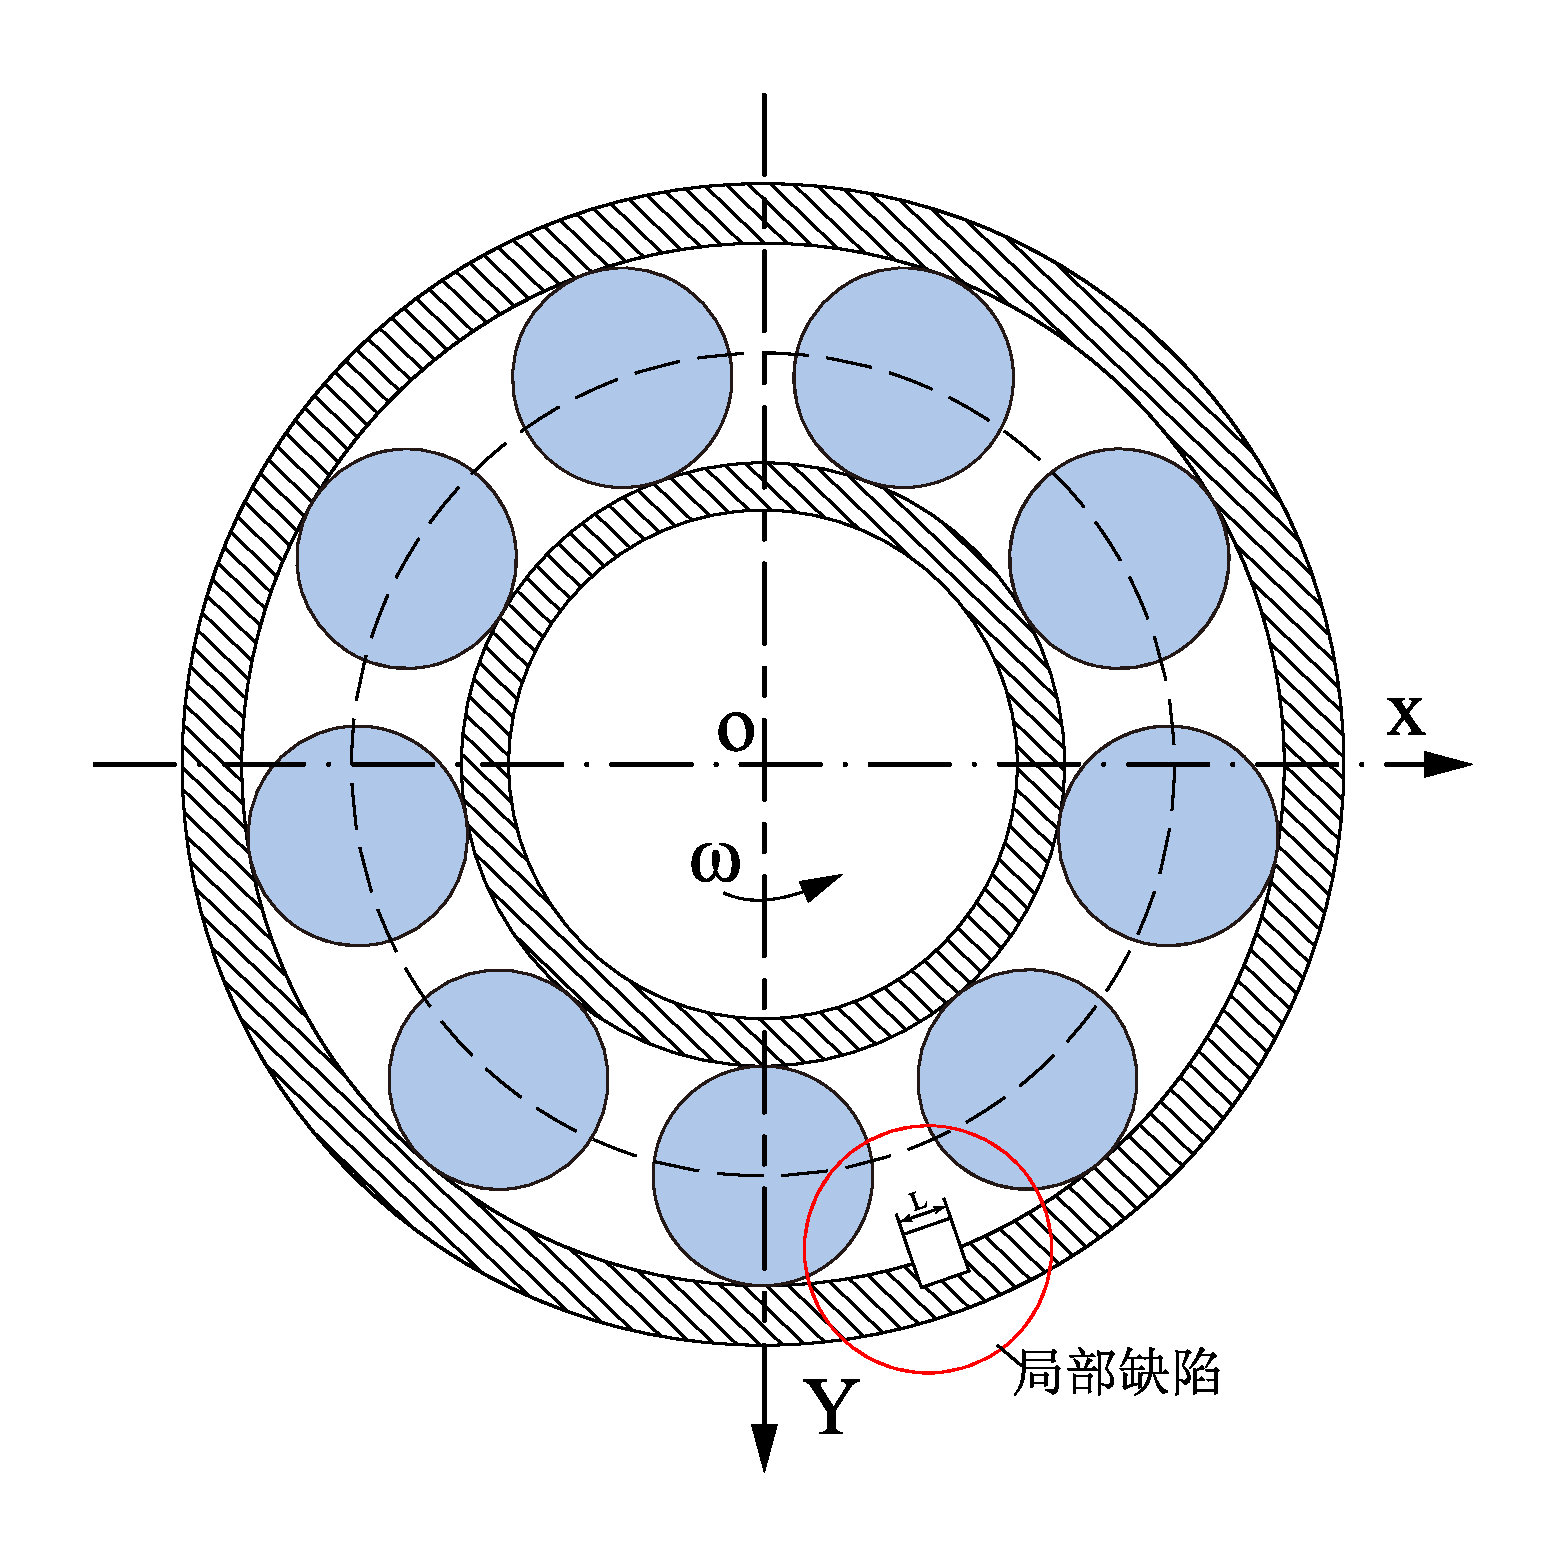
\includegraphics[width=0.45\linewidth]{figures/C3/fig6.pdf}}
	\subcaptionbox{局部几何缺陷俯视图和侧视图\label{fig:subfig-b}}
	{\includegraphics[width=0.45\linewidth]{figures/C3/fig5-1.pdf}}
	%  \caption{局部缺陷}
\end{figure}

% \begin{figure}
	%   \centering
	%   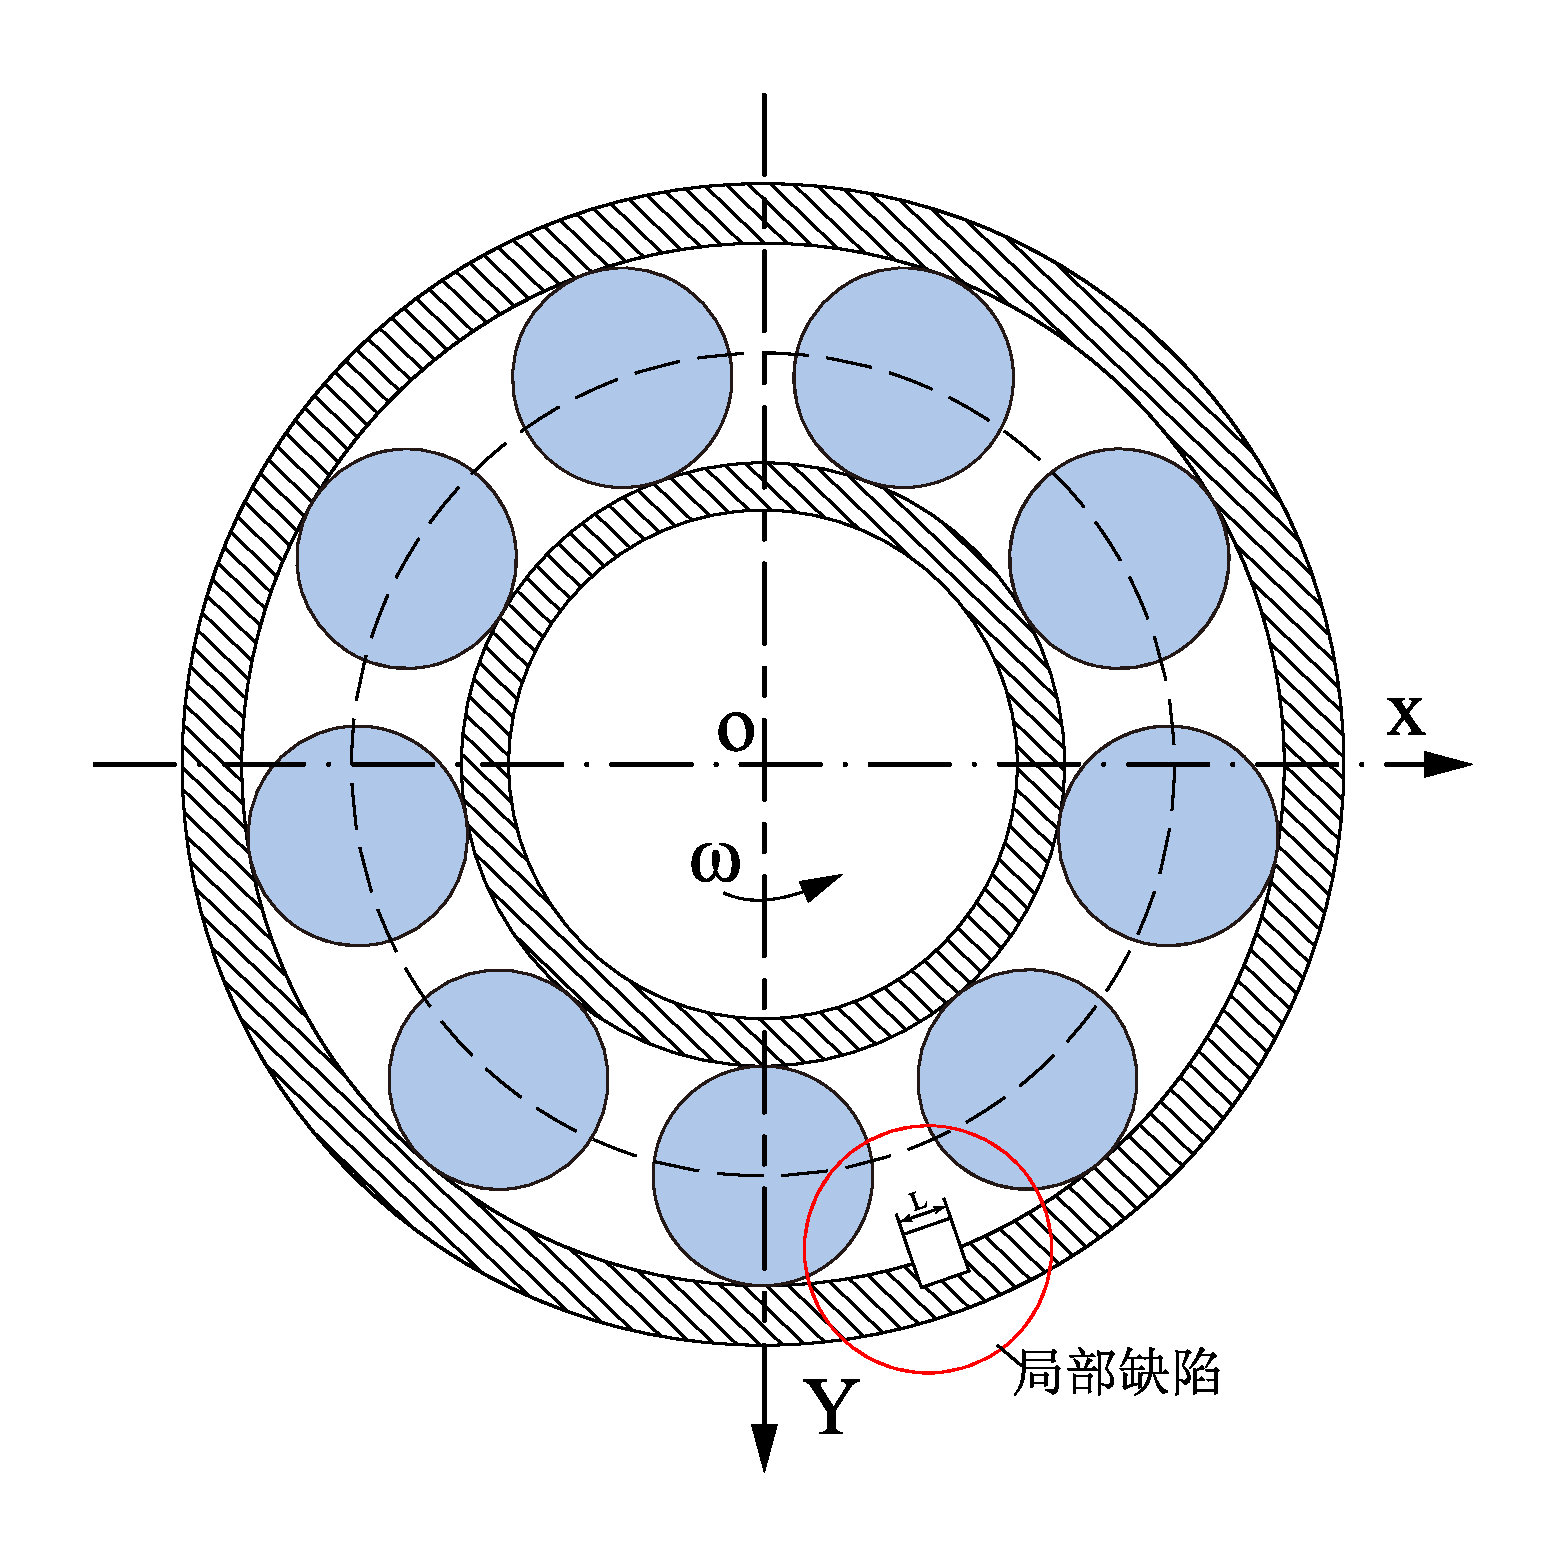
\includegraphics[width=0.5\linewidth]{figures/C3/fig6.pdf}
	%   \caption{外圈上的局部缺陷}
	%   \label{fig:外圈局部缺陷}
	% \end{figure}

% 当滚动轴承滚道表面存在局部缺陷时,以外圈局部故障为例,首先使用直径$L$和深度$H$定义凹痕的物理性质,其故障位置的几何关系如图~\ref{fig:故障俯视图和侧视图}所示。
% \begin{figure}
	%   \centering
	%   \includegraphics[width=0.6\linewidth]{figures/Chap02fig/fig5.png}
	%   \caption{局部几何缺陷俯视图和侧视图}
	%   \label{fig:故障俯视图和侧视图}
	% \end{figure}

球在正常滚道上运动时,其弹性形变$\delta_j$将不会发生变化,只有当其运动到缺陷位置时,弹性形变$\delta_j$会由于接触变化而产生变化,从而影响了轴承的运动。在上一节中已经阐明,根据Hertz接触理论,球与内外圈之间属于点接触,其载荷-弹性形变关系式如下式所示:

当球在正常的滚道上滚动时,其弹性形变
$\delta_j$ 是恒定的,不会有变化。但是,当球滚动至某个有缺陷的位置时,接触情况发生变化,导致弹性形变
$\delta_j$ 随之改变,进而影响了轴承的整体运动。正如前文所述,基于Hertz接触理论,球与内、外圈的接触是点对点的,其载荷与弹性形变之间的关系可以表示为以下公式:
\begin{equation}
	F_j=K_j \delta_j^{n}
\end{equation}

在给定的公式中,符号$n$代表载荷-变形指数,这一指数与缺陷的大小直接相关。考虑到早期的凹痕通常相对较小,并且与球和滚道的整体尺寸相比显得较为微小,我们可以在此环境下合理地假设凹痕的特定几何形状和材料特性的影响可以忽略不计。因此,在这种情境下,Hertz接触的刚度$K$和载荷-变形指数
$n$被认为不受凹痕的影响,而是由缺陷的尺寸来决定其对球运动的主导作用。特别地,对于球,它的载荷-变形指数为$n=1.5$。故其Hertz接触力的计算仍如式~\eqref{eq:elastic deformation}所示。


在本文中,我们采用了分段函数来描述球经过缺陷时的运动行为和建模策略。鉴于早期的缺陷往往相对较小,因此我们没有详细探讨大型缺陷所引入的复杂分段函数模型。我们专注于考虑球的尺寸大于缺陷的尺寸,且这个缺陷是一个长方形,其长度明显大于其宽度的情况。如图~\ref{fig:球与局部缺陷接触关系示意图}所示。
\begin{figure}
	\centering
	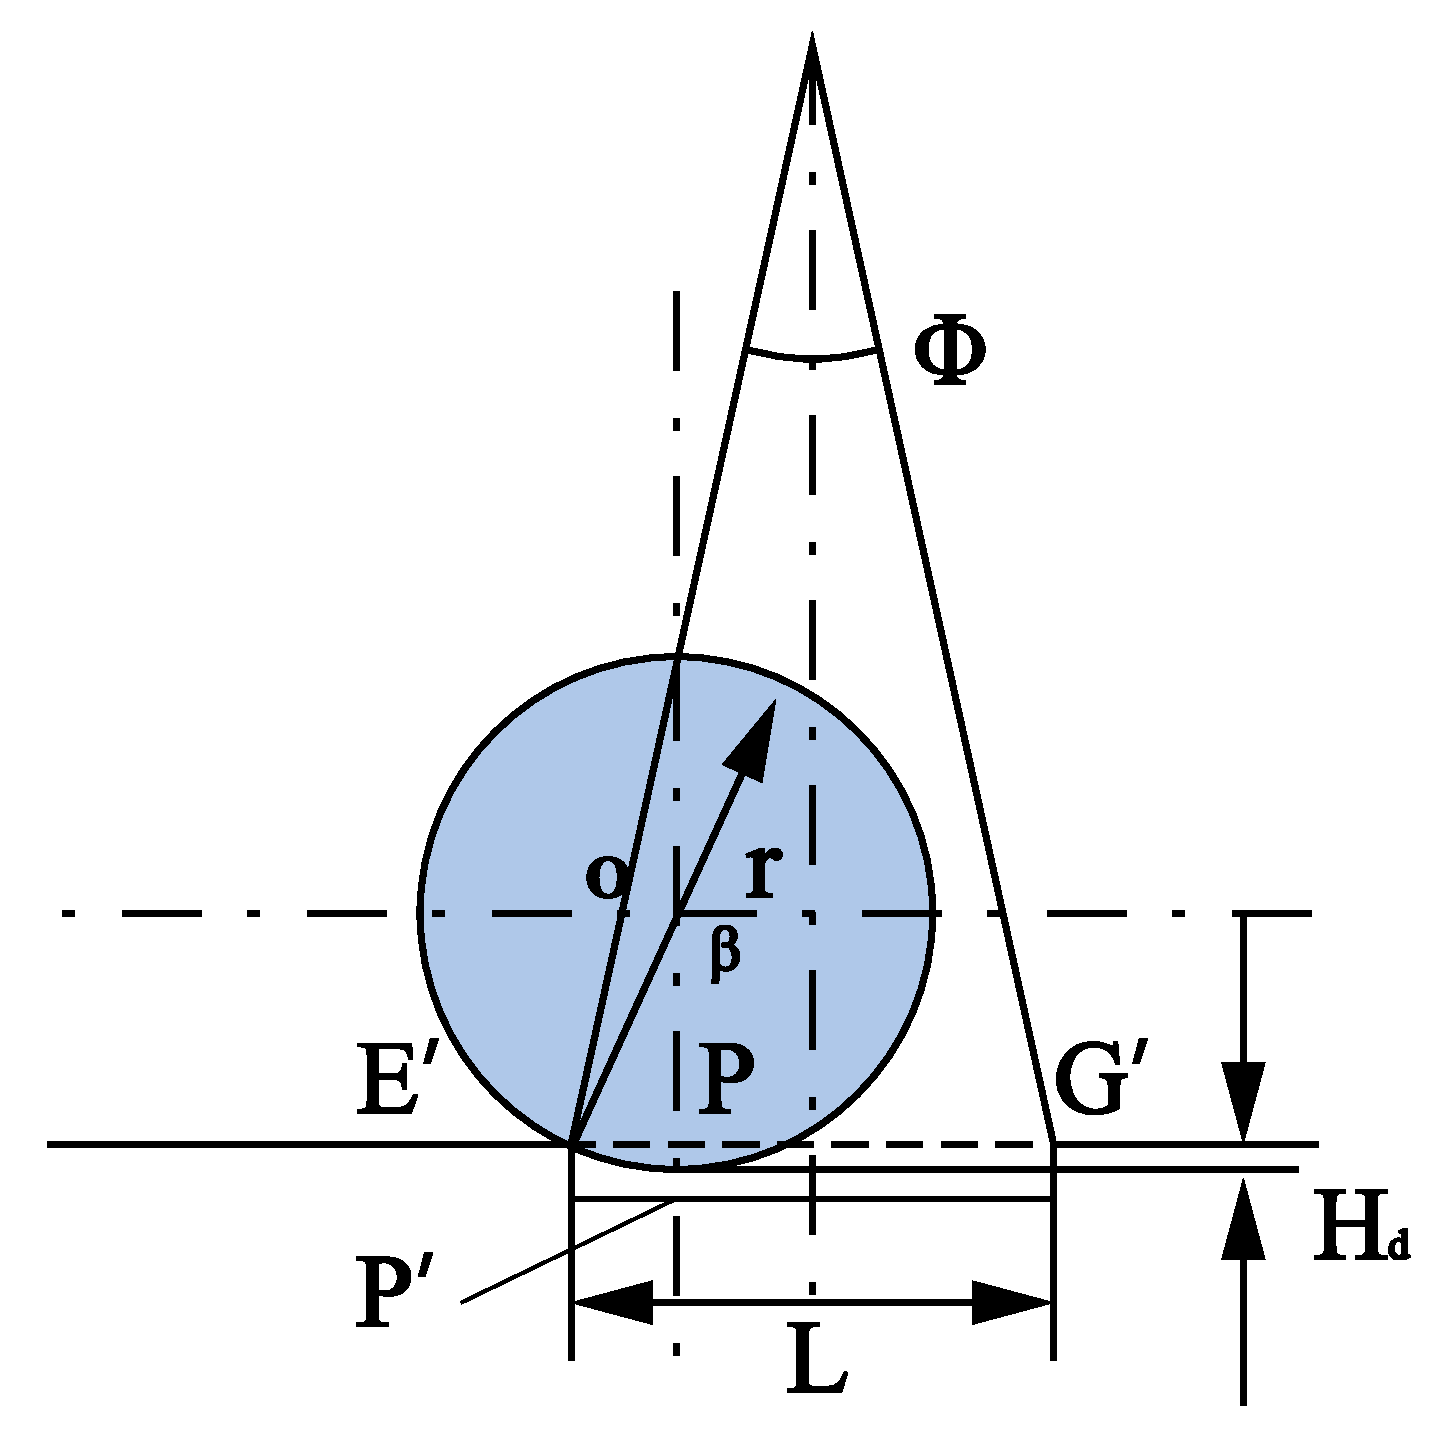
\includegraphics[width=0.3\textwidth]{figures/C3/fig8.pdf}
	\caption{球与局部缺陷接触关系示意图}
	\label{fig:球与局部缺陷接触关系示意图}
\end{figure}

当球经过故障区域时的接触行为可以描述为以下几个步骤:首先,球开始与缺陷的起始边产生接触,并随后与其两侧边产生总计三个接触点;接着,球从缺陷的起始边脱离,仍然与其侧边保持接触,但尚未接触到缺陷的终止边,此时只有两个接触点;最后,当球即将到达缺陷的结束边时,其接触状态与进入缺陷时的状态相似,又重新形成三个接触点。随后,球将返回到正常的滚道上,恢复其正常的滚动状态。具体的接触过程如图~\ref{fig:接触过程示意图}所示。
\begin{figure}[h]
	\centering
	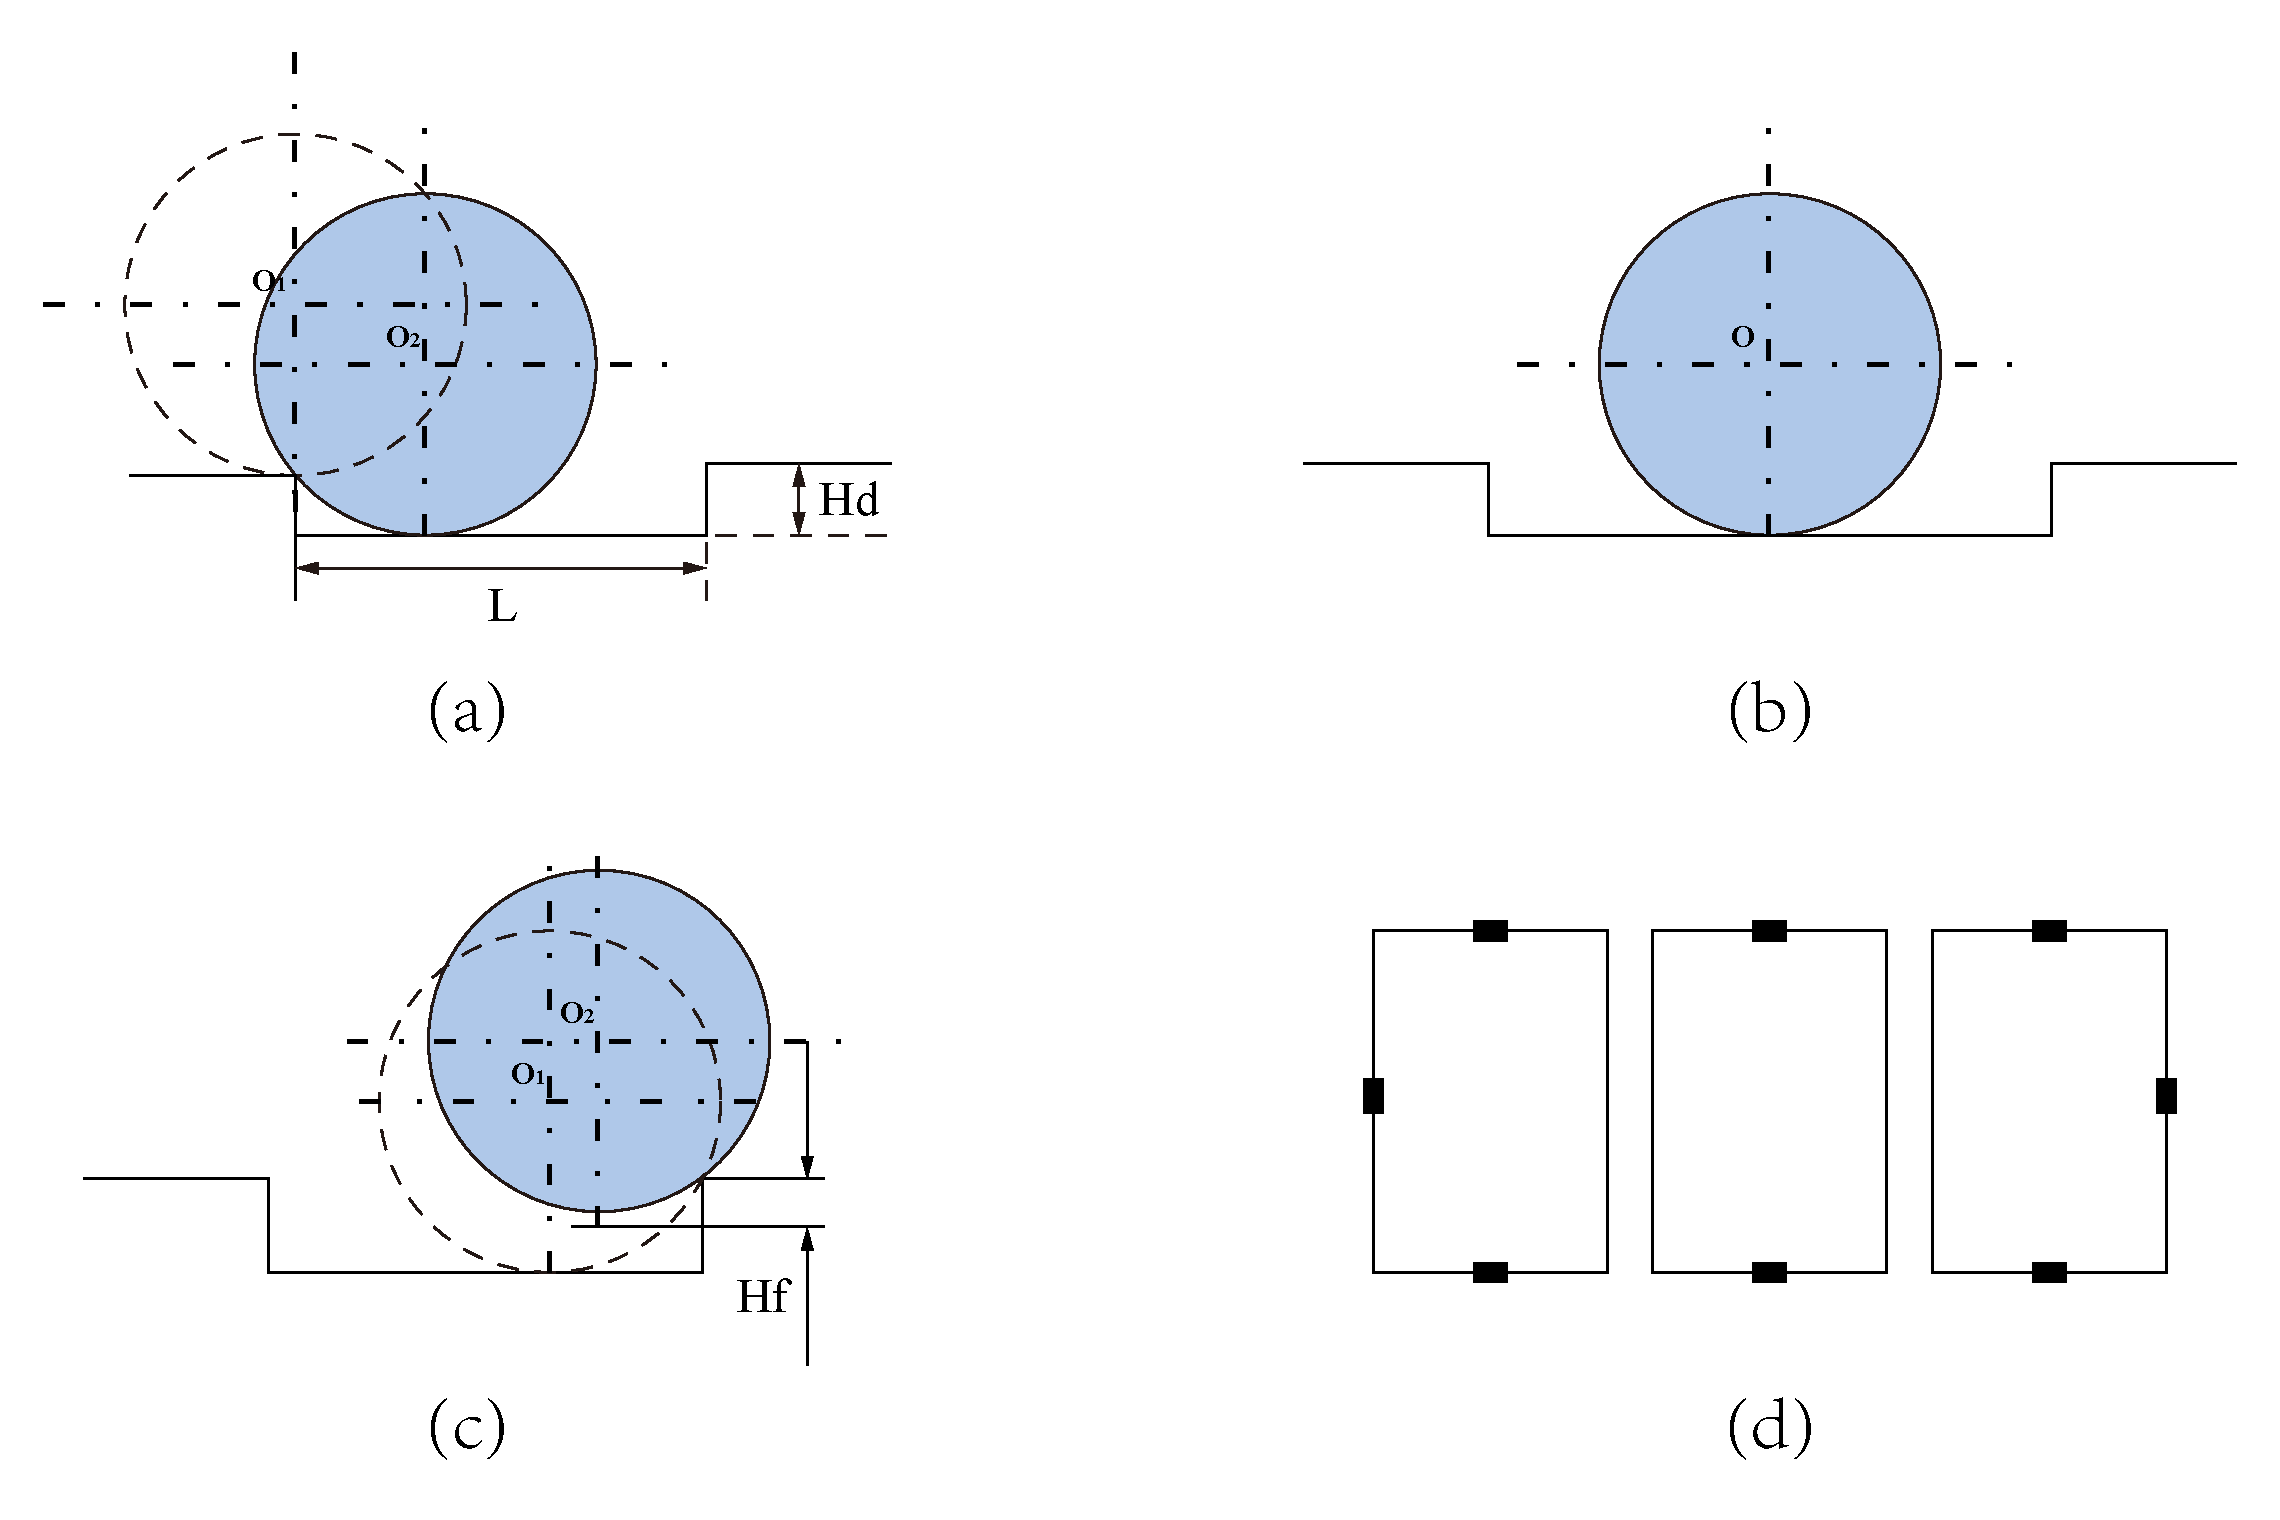
\includegraphics[width=0.7\linewidth]{figures/C3/fig9.pdf}
	\caption{接触过程示意图}
	\label{fig:接触过程示意图}
\end{figure}

基于以上的分析可构造出分段函数模型,如图~\ref{fig:分段函数}所示。
\begin{figure}
	\centering
	\includegraphics[width=0.6\linewidth]{figures/C3/fig7partfunction.png}
	\caption{分段函数示意图}
	\label{fig:分段函数}
\end{figure}

定义轴承中第$j$球的实时角度为:
\begin{equation}
	\phi_{r j}=\bmod \left(\phi_j, 2 \pi\right)
\end{equation}
式子中$\bmod(.)$表示为取余函数。

弹性形变$\delta_j$的变化主要是来源于球与局部缺陷的接触的消失及恢复,当引入故障后,其新的位移可以具体地表达出来:
\begin{equation}
	H_{f j}=\left\{\begin{array}{lc}
		H_d \sin \left(\frac{\pi \cdot \phi_{r j}-\phi_0}{2 \Delta T}\right) & \phi_0 \leq \phi_{r j} \leq \phi_0+\phi_f \\
		0 & \text { otherwise }
	\end{array}\right.
\end{equation}
其中,$\phi_0$是缺陷的初始角度,$\phi_f$是缺陷占据的角度,$\Delta T$是缺陷占据的时间。$H_d$是球进入缺陷区域后接触变形的变化量,即滚道与球圆心距的变化量。其最大值是缺陷的深度$H$,但是一般而言故障早期的缺陷深度$H$远小于球的直径,因此$H_d$可以由下式计算得出:
\begin{equation}
	H_d=0.5 d-\left[(0.5 d)^2-(0.5 W)^2\right]^{0.5}
\end{equation}

另外由于缺陷可能出现在外滚道或内滚道,其表达式可以用下式表示为:
\begin{equation}
	\Delta T=\left\{\begin{array}{l}
		\arcsin \left(\frac{L}{D_0}\right) \\
		\arcsin \left(\frac{L}{D_i}\right)
	\end{array}\right.
\end{equation}
因此最终的有缺陷的弹性变形$\delta_j$表示为:
\begin{equation}
	\delta_j^{\prime}=\delta_j-H_{f j}
\end{equation}

则局部缺陷球轴承在$X$和$Y$方向的总接触力分别表示为: 
\begin{equation}
	\begin{aligned}
		& F_x^{\prime}=\sum_{j=1}^z K \varsigma_j \delta_{e j}^{1.5} \cos \phi_j \\
		& F_y^{\prime}=\sum_{j=1}^z K \varsigma_j \delta_{e j}^{1.5} \sin \phi_j
	\end{aligned}
\end{equation}
其中,$\varsigma_j$为第$j$个球的载荷区系数,其表达式为:
\begin{equation}
	\zeta_j= \begin{cases}1 & \delta_j^{1.5}>0 \\ 0 & \delta_j^{1.5} \leq 0\end{cases}
\end{equation}
$\delta_{e j}$为第 $j$个球的总接触变形,其表示为:
\begin{equation}
	\delta_{e j}=x \cos \theta_j+y \sin \theta_j-\gamma-u_{b j}-H_{f j}
\end{equation}

基于二自由度正常球轴承动力学模型,同时考虑本节的局部缺陷引入的时变位移激励模型,则局部缺陷球轴承的二自由度动力学方程表示为:
\begin{equation}
	\label{eq2:dynamics}
	\begin{aligned}
		& m \ddot{x}+c_x \dot{x}+\sum_{j=1}^Z K_e \varsigma_j\left(x \cos \theta_j+y \sin \theta_j-\gamma-H^{\prime}\right)^{1.5} \cos \theta_j=F_r \\
		& m \ddot{y}+c \dot{y}+\sum_{j=1}^Z K_e \varsigma_j\left(x \cos \theta_j+y \sin \theta_j-\gamma-H^{\prime}\right)^{1.5} \sin \theta_j=mg
	\end{aligned}
\end{equation}
\subsubsection{仿真实验}


为了验证轴承动力学模型的可靠性和实用性,一般会进行实验验证。在这些实验中,通过观察轴承系统的运动、振动和其他相关物理参数,我们可以对动力学模型中的参数和特性进行调整和确认。

根据该模型,当轴承处于完全健康状
态时,轴承时域图和频谱图中理论上不会出现冲击成分,轴承的运转基本处于平
稳状态。首先对一个理想的6205 深沟球轴承进行了动力学响应的研究,该轴承没有滑
动和轴承座的影响。还通过西储大学的轴承实验平台对无故障和无轴承座的6205
深沟球轴承进行试验,以验证我们所建立的二自由度模型的准确性。通过这些实
验,可以更加确信所建立的动力学模型可以准确地预测轴承的动态响应。

图\ref{fig:正常轴承动力学模型求解图}展示了根据四阶龙格库塔方程得出的模拟信号,包括$Y$轴方向的速度、
加速度以及$Y$轴方向的速度、加速度。图\ref{fig:平稳振动信号}则是正常轴承的振动信号的时域图,可
以看出求解出的模拟信号处于周期稳定状态,没有出现较大的冲击成分。图\ref{fig:振动信号频率图}则
是根据图\ref{fig:平稳振动信号}的信号进行快速傅里叶变换得到的频域图。从频谱中可以看出,在轴
承运转初期,轴承处于不稳定状态,振动波动较大,这与实际机器刚启动时的运行
情况相符。根据前文的仿真实验数据,我们可以得知模拟信号的转速为30 Hz。
\begin{figure}
	\centering
	\includegraphics[width=0.65\textwidth]{figures/C3/10.png}
	\caption{正常轴承动力学模型求解图}
	\label{fig:正常轴承动力学模型求解图}
\end{figure}

\begin{figure}[h]
	\centering
	\includegraphics[width=0.65\textwidth]{figures/C3/12.png}
	\caption{平稳振动信号}
	\label{fig:平稳振动信号}
\end{figure}
\begin{figure}[h]
	\centering
	\includegraphics[width=0.65\textwidth]{figures/C3/13.png}
	\caption{振动信号频率图}
	\label{fig:振动信号频率图}
\end{figure}

\subsection{支撑架断裂失效分析}
在扫描电镜的观察下,我们发现了轴承支架上最为显著的两个特征。第一种特征表现为第一张图片中的凹坑,而第二种特征则是支撑架表面的塑性变形。我们基于对轴承使用环境的理解做出了推测,这些凹坑可能是由于轴承在长时间运转过程中受到重复应力的影响,导致了塑性变形。另一种可能的原因是点蚀或异物侵入所致。

图\ref{fig:huan10}中展示了我们对裂纹局部的拍摄结果。同样,我们可以观察到裂纹尖端出现了塑性变形,并呈现出一些类似韧窝的结构。结合轴承的具体使用工况,如果持续运转,在周期性的重复应力作用下,裂纹可能会不断扩展。因此,我们推断该轴承可能的失效形式是疲劳断裂。

球形滚珠轴承支撑架表面出现大量凹坑可能由多种原因引起,其中一些可能的原因包括:

\begin{enumerate}
	\item \textbf{颗粒污染:} 在工作环境中存在颗粒,例如尘土、金属屑等,这些颗粒在滚珠轴承支撑架表面运动时可能引起摩擦和划痕,导致凹坑的形成。
	
	\item \textbf{润滑不足:} 如果润滑油或润滑脂不足,轴承支撑架表面可能会由于摩擦而受损。缺乏足够的润滑可能导致摩擦加剧,从而加速凹坑的形成。
	
	\item \textbf{负荷过重:} 过大的负荷可能会导致滚珠轴承支撑架表面局部应力集中,增加摩擦和磨损的风险,从而引起凹坑。
	
	\item \textbf{表面疲劳:} 长时间高频次的载荷和振动可能导致支撑架表面的疲劳,进而形成凹坑。
	
	\item \textbf{不良制造工艺:} 制造过程中的缺陷或不良工艺可能导致轴承支撑架表面质量不佳,容易受到外部环境的影响而形成凹坑。
	
	\item \textbf{工作条件恶劣:} 若轴承工作在恶劣的环境条件下,如高温、腐蚀性气体等,支撑架表面的保护层可能受到破坏,从而加速凹坑的形成。
\end{enumerate}

通过图\ref{fig:huan21}和图\ref{fig:huan22}所演示的支撑架表面的裂纹扩展和表面结构,我们收集和分析裂裂纹可能形成的原因如下:
\begin{enumerate}
	\item \textbf{疲劳应力:} 滚动轴承在运转过程中会受到周期性的载荷,导致轴承材料经历循环应力。这些循环应力会在轴承材料中形成疲劳区域,从而促使裂纹的扩展。
	\item \textbf{载荷周期性变化:} 滚动轴承在运转中会受到来自旋转和负载的周期性变化,这导致裂纹在负载循环中逐渐扩展,形成波浪形结构。
\end{enumerate}

韧窝结构的形成原因:
\begin{enumerate}
	\item \textbf{局部塑性变形:} 轴承支撑架在运转中可能经历局部的塑性变形,尤其是在受到高频次、高振幅的载荷时。这导致裂纹尖端形成韧窝结构,表现为微小的凹槽和凸起。
	\item \textbf{疲劳扩展:} 韧窝结构也与疲劳断裂过程中裂纹的扩展有关。裂纹扩展时,裂纹尖端的形态会受到材料的塑性变形和撕裂的影响,形成韧窝状结构。
\end{enumerate}

\begin{figure}[!ht]
	\centering
	\subfloat[支撑架表面大量凹坑]{
		\includegraphics[width=0.3\linewidth]{figures/C3/huan10.png}
		\label{fig:huan10}
	}
	\subfloat[支撑架表面塑性形变]{
		\includegraphics[width=0.3\linewidth]{figures/C3/huan21.png}
		\label{fig:huan21}
	}
	\subfloat[支撑架表面裂纹形成]{
		\includegraphics[width=0.3\linewidth]{figures/C3/huan22.png}
		\label{fig:huan22}
	}
	\label{fig:扫描电镜图}
\end{figure}



%\subsection{断口材料分析}
%\subsubsection{滚动轴承材料的主要元素含量及作用}
%
%滚动轴承的性能受其材料成分和含量的显著影响。内圈的滚动轴承通常使用高碳铬轴承钢(GCr15,按照国标GB/T18254-2016制定)。这种钢材的主要成分涵盖碳、铬、硅、锰、钼、磷和硫等元素。接下来,我们将探讨这些元素的含量及其在材料中的作用。
%\begin{table}[h]
%	\caption{高碳铬轴承钢GCr15主要元素含量} 
%	\begin{tabular}{|llllllll|}
%		\hline                                                                                   
%		\multicolumn{1}{|l|}{\textbf{元素}} & \multicolumn{1}{l|}{C}         & \multicolumn{1}{l|}{Cr}        & \multicolumn{1}{l|}{Mn}        & \multicolumn{1}{l|}{Si}        & \multicolumn{1}{l|}{Mo}   & \multicolumn{1}{l|}{P}      & S      \\ \hline
%		\multicolumn{1}{|l|}{\textbf{含量}} & \multicolumn{1}{l|}{0.95-1.05} & \multicolumn{1}{l|}{1.30-1.65} & \multicolumn{1}{l|}{0.20-0.40} & \multicolumn{1}{l|}{0.15-0.35} & \multicolumn{1}{l|}{<0.1} & \multicolumn{1}{l|}{<0.027} & <0.020 \\ \hline
%	\end{tabular}
%\end{table}
%
%1.碳(C): 碳是轴承钢中的关键成分,直接影响其硬度和耐磨特性。不适当的碳浓度可能导致轴承性能下降。
%
%2.铬(Cr): 铬是增强轴承钢硬度和耐磨特性的核心元素。它还增强了钢材的抗腐蚀和抗氧化能力。
%
%3.锰(Mn): 锰提升轴承钢的硬度和强度,并增加其抗磨和抗疲劳性。
%
%4.硅(Si): 硅在轴承钢中起到稳定奥氏体和提高韧性的作用,同时也有助于提升钢的抗氧化性。
%
%5.钼(Mo): 钼能够提升轴承钢的硬度和韧性,进而增强其抗磨和抗疲劳性。
%
%6.磷(P)与硫(S): 这两者在轴承钢中属于不利元素,可能降低其整体韧性和耐磨性。因此,控制这两种元素的浓度是关键。
%
%此外,轴承钢中可能还包含微量的镍、钴和钒等其他合金元素,以进一步优化其性能,但这些通常是较小的成分。
%
%
%
%\subsubsection{滚动轴承外圈磨损面元素分析}
%
%
%从提供的轴承外圈EDS扫描图\ref{fig:轴承外圈磨损面EDS扫瞄图结果}中可以观察到,这些扫描图呈现出异常的钙和氮含量。此现象的原因是,在滚动轴承操作中,钙基润滑剂被引入并在轴承外圈上沉积。随着摩擦产生的热量,这种润滑剂逐渐分解,导致钙和氮化合物沉积在轴承外圈上。此外,高水平的钒、锰和钼可能与热处理过程中这些元素的扩散有关。而在轴承的操作过程中,与其他机器部件的摩擦可能导致金属屑附着在外圈上。最后,轴承在使用中不慎接触外部的杂质和砂粒也可能加剧外圈的磨损情况。
%\begin{figure}[h]
%	\centering
%	\includegraphics[width=1.0\linewidth]{figures/C3/11.jpg}
%	\caption{轴承外圈磨损面EDS扫瞄图结果}
%	\label{fig:轴承外圈磨损面EDS扫瞄图结果}
%\end{figure}


\subsection{分析与总结}


本报告重点是构建滚动轴承的二自由度动力学模型,以模拟其在正常和局部故障工况下的振动行为。开始时,为了简化和便于计算,对轴承系统进行了简化,并制定了必要的假设。在考虑轴承波纹度和应用Hertz接触理论的背景下,成功地构建了正常工作状态下的轴承动力学模型。接着,基于这一正常模型,我们加入了局部故障元素并以规则的几何形状来描述,详细研究了不同的几何参数对轴承振动的影响。通过引入分段函数来分析故障对振动的具体影响,最终得到了故障状态下的轴承动力学模型。最为关键的是,我们通过仿真实验进行了验证,将仿真振动数据与实验台收集的数据进行了对比分析,包含时域和频域的两个维度。经过对比,我们发现仿真数据能够准确地展现正常和故障状态下的特征,从而确保了所建立轴承动力学模型的精确性和可靠性。同时,从材料的角度来看,滚动轴承的失效可能与不适当的材料选择有关,如果选择的轴承材料不能满足特定应用的需求,例如在高温、高湿或强腐蚀环境下,轴承可能会提前失效或断裂。不恰当的润滑、尘土或杂质进入轴承内部都可能导致过度磨损,进而降低轴承的使用寿命并可能引发断裂。同时过热与化学侵蚀也会导致轴承的失效,轴承在持续高温环境中运行可能导致材料的结构改变,这可能会降低其强度和韧性,进而导致断裂; 轴承材料暴露在化学腐蚀性环境中可能会发生化学侵蚀,这会降低材料的强度并可能导致断裂。












%%------------------------第四章从这里开始-------------------%
\section{解决措施}
当滚动轴承出现断裂后,为确保设备的安全和性能,需要采取一系列的故障诊断和解决措施。以下是针对滚动轴承断裂后的具体解决措施:

首先是短期措施,短期措施的目的在于短时间内确定断裂原因,消除直接隐患,安全地恢复设备运行或防止事态扩大。

(1) 现场故障诊断与根因排查:
利用现有的监测手段,进行全面的故障诊断。通过振动分析,声学分析和温度检测,锁定轴承断裂的具体物理表证。
立即检查断裂轴承的工作环境。核实当时的负荷状态,润滑情况,找出导致断裂的直接诱因。

(2) 润滑系统与维护检查:
检查当前润滑油/脂的清洁度和油位。如果发现由于润滑失效导致的断裂,必须立即清洗润滑管路并更换新的润滑剂,防止残留的金属碎屑对新轴承造成二次伤害。
检查密封件是否破损,防止尘土和杂质继续进入轴承座。

(3)容错控制与安全停机:
如果设备具备关键应用中的冗余设计或备用轴承系统,应立即切换至备用系统,确保设备基本功能的维持。
如果尚未发生灾难性后果,依靠现有的保护机制,强制设备停机,防止断裂的轴承碎片损坏轴、齿轮箱或电机等昂贵部件。

之后是长期措施,长期措施旨在从根本上消除故障隐患,提升设备的智能化水平和机械可靠性,实现“预测性维护”。

(4) 智能化监控与算法升级:
建立早期的预警系统,而不是等到断裂才处理,而是从算法角度设计预警机制。利用实时监测数据,建立健康度模型。一旦检测到微弱的故障特征,立即警告操作员或触发自动保护。
引入自适应控制算法,根据轴承的实时状态动态调整操作参数。例如:在检测到轴承状态恶化时,自动减低转速或减轻负荷,以延长剩余寿命。

(5) 结构优化与材料改进:
重新评估轴承材料,根据工作环境,选择更耐磨、耐腐蚀或耐高温的特种钢材或陶瓷材料。采用先进的材料处理工艺,如表面硬化、渗氮、涂层处理等,显著提高轴承表面的硬度和抗疲劳性能。
重新审查机械设计,优化轴承的载荷分布,减小应力集中区域。必要时改变轴承的支撑结构或安装方式,以降低工作中的振动耦合和冲击载荷。

(6) 制造工艺与运维管理:
如果断裂源于质量缺陷,需引入更严格的供应商管理或生产工艺。利用数字化制造和精密加工技术,确保轴承的一致性和精度。
建立长效的润滑管理制度。优化润滑系统设计,确保润滑油的持续清洁和有效供给。
\section{收尾}
断裂力学与失效分析的课程即将结束,在此对课程与报告进行相应的总结:

(1) 课程理论与实践的结合:在学术课程中学到的理论知识与实际应用之间建立联系是非常令人满足的。通过实际的失效案例研究,我们能够将书本上的知识与实际场景相结合,更深入地理解材料和结构的行为。本次项目完成经过 3次线下集中讨论,修改、整合、完善;

(2) 挑战性与探索性:断裂力学与失效分析涉及多学科的知识,如材料科学、工程力学、化学等。这为我们提供了一个广阔的研究平台,鼓励我们探索和解决实际工程问题。

(3) 责任与重要性:从失效分析中,我们意识到材料和结构在工程应用中的重要性。正确的材料选择、设计和维护对于确保设备的安全和性能至关重要。这为我们未来的工作提供了一个明确的方向和责任感。

(4) 项目的顺利完成,离不开朱强老师的指导和朱老师课题组卢老师、徐老师和几位助教师兄师
姐的帮助,以及每位项目组成员的辛勤努力与付出。

总的来说,学习断裂力学与失效分析是一个充满挑战和机会的过程。它不仅增强了我们的技术能力,还培养了我们的批判性思维、问题解决能力和职业素养,为我们未来的职业生涯奠定了坚实的基础。

\section{参考文献}
\noindent{[1] KONG X, LI S, WANG E, et al. Dynamics behaviour of gas-bearing coal subjected to SHPB
	tests[J]. Composite Structures, 2021, 256: 113088. }

\noindent{[2] CAO H, NIU L, XI S, et al. Mechanical model development of rolling bearing-rotor systems:
	A review[J]. Mechanical Systems and Signal Processing, 2018, 102: 37-58.}

\noindent{[3] OHTA H, SUGIMOTO N. Vibration characteristics of tapered roller bearings[J]. Journal of
	Sound and vibration, 1996, 190(2): 137-147.}

\noindent{[4] 庞彬. 基于奇异谱分解的旋转机械故障诊断研究[D]. 北京: 华北电力大学(北京), 2020.}

\noindent{[5] 张梅军. 机械状态监测测与故障诊断[M]. 北京: 国防法学出版社, 2008.}

\noindent{[6] 杨晨. 强噪声背景下多工况、多故障模式的滚动轴承故障诊断研究[D]. 北京: 中国矿业大学,
	2021.}

\noindent{[7] 庄絮竹. 基于振动分析的变转速工况滚动轴承故障诊断研究[D]. 北京: 中国矿业大学, 2022.}


\noindent{[8] STACKE L E, FRITZSON D. Dynamic behaviour of rolling bearings: simulations and experiments[
	J]. Proceedings of the Institution of Mechanical Engineers, Part J: Journal of Engineering
	Tribology, 2001, 215(6): 499-508.}

\noindent{[9] HAN Q, LI X, CHU F. Skidding behavior of cylindrical roller bearings under time-variable
	load conditions[J]. International Journal of Mechanical Sciences, 2018, 135: 203-214.}

\noindent{[10] SELVARAJ A, MARAPPAN R. Experimental analysis of factors influencing the cage slip in
	cylindrical roller bearing[J]. The International Journal of Advanced Manufacturing Technology,
	2011, 53: 635-644.}

\noindent{[11] WANG Y, WANG W, ZHANG S, et al. Investigation of skidding in angular contact ball bearings
	under high speed[J]. Tribology International, 2015, 92: 404-417.}

\noindent{[12] 张忠云, 吴建德, 马军, 等. 基于混沌分形理论的滚动轴承微小故障诊断[J]. 中南大学学报
	(自然科学版), 2016, 47(02): 640-6.}

\noindent{[13] Li Y. Study on Incipient Fault Diagnosis for Rolling Bearings Based on Wavelet and Neural
	Networks[C]. International Conference on Natural Computation: IEEE, 2008.}

\noindent{[14] Zheng K, Luo J, Zhang Y, et al. Incipient fault detection of rolling bearing using maximum
	autocorrelation impulse harmonic to noise deconvolution and parameter optimized fast EEMD[J].
	ISA Transactions, 2019, 89: 256-71.}




\end{document}